% ============================================================
% SIGA-Óptica — Defensa de Trabajo Final de Grado
% Presentación Beamer — 20 minutos, dos expositores.
% Compilar con pdfLaTeX (mismo motor que la tesis).
% Las imágenes se toman de ../imagenes/ (no se duplican).
% ============================================================

\documentclass[11pt,aspectratio=169]{beamer}

\usepackage[utf8]{inputenc}
\usepackage[T1]{fontenc}
\usepackage{lmodern}
\usepackage[spanish]{babel}
\AtBeginDocument{\shorthandoff{<>}}

\usepackage{graphicx}
\usepackage{booktabs}
\usepackage{tikz}
\usetikzlibrary{positioning,arrows.meta,shapes.multipart,calc,fit,backgrounds}

% ---------- Paleta institucional (idéntica a la tesis) ----------
\definecolor{sigaAzul}{HTML}{00288E}
\definecolor{sigaCyan}{HTML}{006780}
\definecolor{sigaVerde}{HTML}{1B7A3D}
\definecolor{sigaAmbar}{HTML}{9A6700}
\definecolor{sigaRojo}{HTML}{B3261E}
\definecolor{sigaGris}{HTML}{5F6368}

% ---------- Tema: limpio, sin adornos ----------
\usetheme{default}
\usecolortheme{default}
\setbeamertemplate{navigation symbols}{}
\setbeamercolor{structure}{fg=sigaAzul}
\setbeamercolor{frametitle}{fg=sigaAzul}
\setbeamercolor{title}{fg=sigaAzul}
\setbeamerfont{frametitle}{series=\bfseries,size=\large}
\setbeamerfont{title}{series=\bfseries,size=\LARGE}
\setbeamertemplate{itemize item}{\color{sigaAzul}$\blacktriangleright$}
\setbeamertemplate{itemize subitem}{\color{sigaGris}--}
\setbeamercolor{block title}{bg=sigaAzul!12,fg=sigaAzul}
\setbeamercolor{block body}{bg=sigaAzul!4}
\setbeamercolor{alerted text}{fg=sigaCyan}

% Línea fina bajo el título de cada diapositiva
\setbeamertemplate{frametitle}{%
  \vspace{6pt}%
  \usebeamerfont{frametitle}\usebeamercolor[fg]{frametitle}\insertframetitle\par
  \vspace{-4pt}%
  {\color{sigaAzul!35}\rule{\textwidth}{0.8pt}}\par
  \vspace{2pt}%
}

% Pie: sección · expositor · número de diapositiva
\setbeamertemplate{footline}{%
  \hbox{%
    \begin{beamercolorbox}[wd=.72\paperwidth,ht=2.4ex,dp=1.2ex,leftskip=1em]{}%
      {\scriptsize\color{sigaGris}SIGA-Óptica \textbullet\ \insertsection}%
    \end{beamercolorbox}%
    \begin{beamercolorbox}[wd=.28\paperwidth,ht=2.4ex,dp=1.2ex,rightskip=1em]{}%
      \hfill{\scriptsize\color{sigaGris}\insertframenumber\,/\,\inserttotalframenumber}%
    \end{beamercolorbox}%
  }%
  \vspace{2pt}%
}

% Diapositiva de sección, con el expositor a cargo
\newcommand{\seccion}[2]{%
  \begin{frame}[plain]
    \vfill
    \begin{center}
      {\color{sigaAzul!30}\rule{0.5\textwidth}{1pt}}\\[10pt]
      {\LARGE\bfseries\color{sigaAzul}#1}\\[10pt]
      {\color{sigaAzul!30}\rule{0.5\textwidth}{1pt}}\\[14pt]
      {\small\color{sigaGris}#2}
    \end{center}
    \vfill
  \end{frame}%
}

% Estilos TikZ heredados de la tesis
\tikzset{
  capa/.style={rectangle, rounded corners, draw=sigaAzul, thick,
    fill=sigaAzul!8, minimum width=2.4cm, minimum height=1.0cm,
    align=center, font=\scriptsize},
  externo/.style={rectangle, draw=sigaGris, thick, fill=sigaGris!10,
    minimum width=2.2cm, minimum height=0.85cm, align=center, font=\scriptsize},
  entidad/.style={rectangle split, rectangle split parts=2, draw=sigaAzul,
    thick, rectangle split part align={center,left}, rounded corners=1pt,
    fill=white, font=\scriptsize, text width=2.5cm, align=left, inner sep=3pt},
  flechaArq/.style={-{Latex[length=2mm]}, thick, sigaGris},
  relacion/.style={-, thick, sigaGris},
}

% ---------- Datos de portada ----------
\title{SIGA-Óptica}
\subtitle{Sistema Integral de Gestión y Agendamiento para Ópticas}
\author{Matías Melgarejo \and Matías Gaona}
\institute{Universidad Nacional de Asunción \\ Facultad Politécnica \\ Licenciatura en Ciencias Informáticas}
\date{San Lorenzo --- 2026}

\begin{document}

% ============================================================
{\setbeamertemplate{footline}{}
\begin{frame}[plain]
  \vfill
  \begin{center}
    {\LARGE\bfseries\color{sigaAzul}SIGA-Óptica\par}
    \vspace{4pt}
    {\large Sistema Integral de Gestión y Agendamiento para Ópticas\par}
    \vspace{2pt}
    {\small\color{sigaGris}Defensa de Trabajo Final de Grado\par}
    \vspace{18pt}
    {\color{sigaAzul!30}\rule{0.45\textwidth}{0.8pt}}
    \vspace{14pt}

    \begin{tabular}{rl}
      \small\textbf{Autores:} & \small Matías Melgarejo \\
                              & \small Matías Gaona \\[4pt]
      \small\textbf{Tutores:} & \small Prof. Lic. Diego Ruiz Diaz \\
                              & \small Lic. Juan Fernando Dure \\
    \end{tabular}

    \vspace{16pt}
    {\footnotesize\color{sigaGris}Universidad Nacional de Asunción --- Facultad Politécnica\\
    Licenciatura en Ciencias Informáticas --- San Lorenzo, 2026\par}
  \end{center}
  \vfill
\end{frame}}

% ============================================================
\begin{frame}{Contenido}
  \begin{columns}[T,onlytextwidth]
    \begin{column}{0.48\textwidth}
      {\color{sigaGris}\small\textbf{Primera parte}}\\[4pt]
      \begin{enumerate}
        \item El problema
        \item Objetivos del proyecto
        \item La solución y su arquitectura
        \item Decisiones de diseño clave
      \end{enumerate}
    \end{column}
    \begin{column}{0.48\textwidth}
      {\color{sigaGris}\small\textbf{Segunda parte}}\\[4pt]
      \begin{enumerate}
        \setcounter{enumi}{4}
        \item El sistema construido
        \item Cambios respecto al anteproyecto
        \item Validación
        \item Conclusiones
      \end{enumerate}
    \end{column}
  \end{columns}
\end{frame}

% ============================================================
\section{El problema}
\seccion{Primera parte}{El problema, la solución y su arquitectura --- Matías Melgarejo}

\begin{frame}{El problema}
  \textbf{Centro Óptico Santa María} --- óptica con consultorio oftalmológico asociado.

  \vspace{8pt}
  Gestionaba su operación con \alert{procesos manuales y herramientas desconectadas}:

  \vspace{6pt}
  \begin{columns}[T,onlytextwidth]
    \begin{column}{0.48\textwidth}
      \begin{itemize}
        \item Agendamiento de citas
        \item Historia clínica de pacientes
      \end{itemize}
    \end{column}
    \begin{column}{0.48\textwidth}
      \begin{itemize}
        \item Control de inventario óptico
        \item Seguimiento de ventas
      \end{itemize}
    \end{column}
  \end{columns}

  \vspace{12pt}
  \begin{block}{Consecuencias}
    Información poco confiable para la atención y para decidir; errores de registro,
    duplicidad de datos y demoras evitables.
  \end{block}
\end{frame}

% ============================================================
\begin{frame}{Objetivo general y objetivos específicos}
  \begin{block}{Objetivo general}
    Desarrollar un sistema web integral que centralice la gestión administrativa,
    clínica y comercial de la óptica en una única plataforma.
  \end{block}

  \vspace{6pt}
  {\small Los cinco objetivos específicos del anteproyecto:}
  \vspace{2pt}
  \begin{enumerate}
    \item Módulo de \textbf{pacientes}: registro, historial clínico e historial de compras.
    \item Módulo \textbf{clínico digital}: consultas, diagnósticos y recetas.
    \item Módulo de \textbf{gestión de óptica}: stock en tiempo real y registro de ventas.
    \item \textbf{Agendamiento en línea} autogestionado por el paciente.
    \item \textbf{Interfaz amigable y accesible}.
  \end{enumerate}
\end{frame}

% ============================================================
\section{La solución}

\begin{frame}{La solución: SIGA-Óptica}
  Sistema web que cubre el \alert{ciclo completo de la óptica}, de punta a punta:

  \vspace{10pt}
  \begin{center}
  \resizebox{\textwidth}{!}{%
  \begin{tikzpicture}[node distance=0pt]
    \node[capa, minimum width=2.0cm, text width=1.9cm] (p) at (0,0)    {Paciente\\\scriptsize registro};
    \node[capa, minimum width=2.0cm, text width=1.9cm] (t) at (2.6,0)  {Turno\\\scriptsize agenda};
    \node[capa, minimum width=2.0cm, text width=1.9cm] (c) at (5.2,0)  {Consulta\\\scriptsize receta};
    \node[capa, minimum width=2.0cm, text width=1.9cm] (v) at (7.8,0)  {Venta\\\scriptsize cobro};
    \node[capa, minimum width=2.0cm, text width=1.9cm] (l) at (10.4,0) {Laboratorio\\\scriptsize a pedido};
    \node[capa, minimum width=2.0cm, text width=1.9cm] (s) at (13.0,0) {Stock\\\scriptsize inventario};
    \draw[flechaArq] (p) -- (t);
    \draw[flechaArq] (t) -- (c);
    \draw[flechaArq] (c) -- (v);
    \draw[flechaArq] (v) -- (l);
    \draw[flechaArq] (v) to[out=-40,in=-140] (s);
  \end{tikzpicture}%
  }
  \end{center}

  \vspace{10pt}
  \begin{itemize}
    \item \textbf{16 módulos de negocio} sobre una base común.
    \item Control de acceso \textbf{por permisos individuales}, no por rol fijo.
    \item Operación \textbf{multi-sucursal} simultánea.
  \end{itemize}
\end{frame}

% ============================================================
\begin{frame}{Stack tecnológico}
  \begin{columns}[T,onlytextwidth]
    \begin{column}{0.48\textwidth}
      \begin{block}{Backend --- \textnormal{repositorio \texttt{SIGA}}}
        \begin{itemize}\small
          \item ASP.NET Core Web API (.NET 10), C\#
          \item Entity Framework Core
          \item PostgreSQL (hosteado en Neon)
          \item Autenticación JWT Bearer
        \end{itemize}
      \end{block}
    \end{column}
    \begin{column}{0.48\textwidth}
      \begin{block}{Frontend --- \textnormal{repositorio \texttt{SIGA-Web}}}
        \begin{itemize}\small
          \item Vue 3 (SPA), TypeScript
          \item Vite
          \item Sistema de diseño propio
          \item Modo claro / oscuro, responsive
        \end{itemize}
      \end{block}
    \end{column}
  \end{columns}

  \vspace{8pt}
  \begin{block}{Despliegue}
    \small Contenedores Docker sobre un VPS Linux (Ubuntu 24.04 LTS), con Caddy
    como proxy inverso y TLS automático. Servicios externos: \textbf{Resend} (email)
    y \textbf{hCaptcha} (antibot).
  \end{block}
\end{frame}

% ============================================================
\begin{frame}{Arquitectura de componentes}
  \begin{center}
  \resizebox{\textwidth}{!}{%
  \begin{tikzpicture}
    \node[capa, minimum width=2.6cm, minimum height=1.4cm, text width=2.4cm] (web)   at (0,0)    {SIGA-Web\\\scriptsize Vue 3 SPA};
    \node[capa, minimum width=2.6cm, minimum height=1.4cm, text width=2.4cm] (api)   at (4.0,0)  {SIGA.Api\\\scriptsize Controllers, JWT, Policies};
    \node[capa, minimum width=2.8cm, text width=2.6cm] (app)   at (7.8,1.5)  {SIGA.Application\\\scriptsize Interfaces, DTOs};
    \node[capa, minimum width=2.8cm, text width=2.6cm] (dom)   at (7.8,-1.5) {SIGA.Domain\\\scriptsize Entities};
    \node[capa, minimum width=2.9cm, minimum height=1.4cm, text width=2.7cm] (infra) at (11.6,0) {SIGA.Infrastructure\\\scriptsize Services, DbContext, Migrations};
    \node[externo] (db)  at (15.0,1.5)  {PostgreSQL};
    \node[externo] (rs)  at (15.0,0)    {Resend};
    \node[externo] (hc)  at (15.0,-1.5) {hCaptcha};

    \draw[flechaArq] (web) -- node[below=0.85cm,font=\scriptsize,align=center]
          {HTTPS REST + JWT} (api);
    \draw[flechaArq] (api) -- (app);
    \draw[flechaArq] (api) -- (dom);
    \draw[flechaArq, dashed] (infra) -- node[font=\scriptsize,pos=0.5,
          fill=white,inner sep=2pt] {implementa} (app);
    \draw[flechaArq] (infra) -- (dom);
    \draw[flechaArq] (infra) -- (db);
    \draw[flechaArq] (infra) -- (rs);
    \draw[flechaArq] (infra) -- (hc);
  \end{tikzpicture}%
  }
  \end{center}

  \vspace{4pt}
  {\small Arquitectura en capas: \texttt{Domain} no depende de nadie;
  \texttt{Infrastructure} \emph{implementa} los contratos que declara
  \texttt{Application} --- inversión de dependencias.}
\end{frame}

% ============================================================
\section{Decisiones de diseño}

\begin{frame}{Decisión 1 --- Autorización por permisos, no por roles}
  \begin{columns}[T,onlytextwidth]
    \begin{column}{0.5\textwidth}
      \textbf{Enfoque habitual}
      \begin{itemize}\small
        \item El token lleva el \emph{rol}.
        \item El endpoint exige un rol concreto.
        \item Un rol nuevo obliga a modificar código y volver a desplegar.
      \end{itemize}
    \end{column}
    \begin{column}{0.5\textwidth}
      \textbf{Enfoque adoptado}
      \begin{itemize}\small
        \item Un rol es solo una \emph{colección con nombre} de permisos.
        \item El token lleva los \textbf{permisos resueltos}.
        \item El endpoint exige un permiso puntual.
      \end{itemize}
    \end{column}
  \end{columns}

  \vspace{10pt}
  \begin{block}{Consecuencia práctica}
    El administrador crea roles a medida desde la propia aplicación
    --- sin modificar código ni volver a desplegar. También puede conceder o
    revocar permisos a un usuario en particular, por encima de su rol.
  \end{block}
\end{frame}

% ============================================================
\begin{frame}{Decisión 2 --- Aislamiento multi-sucursal}
  El sistema opera varias sucursales físicas sobre \alert{una única base de datos},
  garantizando que cada una vea solo lo suyo.

  \vspace{8pt}
  \begin{itemize}
    \item Cada usuario pertenece a una sucursal; el dato viaja en el \textbf{token}.
    \item Las consultas se filtran por sucursal de forma \textbf{transversal},
          no endpoint por endpoint.
    \item Pedir por identificador un recurso de otra sucursal devuelve
          \emph{no encontrado} --- no expone la existencia del dato.
    \item El administrador \emph{sin} sucursal fija conserva visibilidad global.
    \item Operaciones legítimamente compartidas --- como una transferencia de stock
          --- son visibles desde ambas puntas.
  \end{itemize}
\end{frame}

% ============================================================
\begin{frame}{Decisión 3 --- \texttt{Person} como núcleo del modelo}
  Una misma persona puede ser paciente, cliente y empleado a la vez.
  Modelarlas por separado duplicaría sus datos.

  \vspace{6pt}
  \begin{center}
  \resizebox{0.86\textwidth}{!}{%
  \begin{tikzpicture}
    \node[entidad, text width=3.0cm] (per) at (0,0)
      {\textbf{\textcolor{sigaAzul}{Person}} \nodepart{two} CI, nombre, contacto};
    \node[capa, minimum width=2.0cm] (usr) at (-4.5,-2.4) {User\\\scriptsize accede al sistema};
    \node[capa, minimum width=2.0cm] (pat) at (-1.5,-2.4) {Patient\\\scriptsize se atiende};
    \node[capa, minimum width=2.0cm] (pro) at (1.5,-2.4)  {Professional\\\scriptsize atiende};
    \node[capa, minimum width=2.0cm] (cli) at (4.5,-2.4)  {Cliente\\\scriptsize compra};
    \node[capa, minimum width=2.0cm] (emp) at (7.5,-2.4)  {Empleado\\\scriptsize trabaja};
    \foreach \n in {usr,pat,pro,cli,emp}{\draw[relacion] (per.south) -- (\n.north);}
  \end{tikzpicture}%
  }
  \end{center}

  \vspace{4pt}
  {\small Los roles funcionales \emph{se cuelgan} de \texttt{Person} según lo que esa
  persona necesite hacer. Un dato de contacto se corrige en un solo lugar.}
\end{frame}

% ============================================================
\seccion{Segunda parte}{El sistema construido, validación y conclusiones --- Matías Gaona}

\section{El sistema construido}

\begin{frame}{Los 16 módulos entregados}
  \small
  \begin{columns}[T,onlytextwidth]
    \begin{column}{0.33\textwidth}
      {\color{sigaAzul}\textbf{Personas}}
      \begin{itemize}\small
        \item Identidad y acceso
        \item Pacientes y profesionales
        \item Personal
        \item Clientes
        \item Roles y permisos
      \end{itemize}
    \end{column}
    \begin{column}{0.33\textwidth}
      {\color{sigaAzul}\textbf{Atención}}
      \begin{itemize}\small
        \item Agenda de turnos
        \item Historia clínica
        \item Laboratorio óptico
        \item Notificaciones
      \end{itemize}
    \end{column}
    \begin{column}{0.33\textwidth}
      {\color{sigaAzul}\textbf{Comercial}}
      \begin{itemize}\small
        \item Inventario y catálogo
        \item Ventas
        \item Compras
        \item Caja y egresos
        \item Reportes
        \item Sucursales
        \item Auditoría
      \end{itemize}
    \end{column}
  \end{columns}

  \vspace{8pt}
  \begin{block}{Dimensión del sistema}
    \small 37 controllers · 235 endpoints · 96 archivos de entidad ·
    90 migraciones de base de datos · 91 vistas de frontend.
  \end{block}
\end{frame}

% ============================================================
\begin{frame}{El flujo que atraviesa todo: la venta ``a pedido''}
  El caso más completo del sistema, y el que justifica la integración:

  \vspace{8pt}
  \begin{enumerate}
    \item El paciente reserva su \textbf{turno} desde el portal.
    \item El profesional registra la \textbf{consulta} y emite la \textbf{receta óptica}.
    \item Se genera una \textbf{venta} con armazón de stock y cristal a medida.
    \item El cristal se encarga a un \textbf{laboratorio externo}: el pedido se sigue
          por estados hasta su recepción.
    \item Se \textbf{cobra}, se emite el \textbf{comprobante fiscal} y se descuenta
          el \textbf{stock} consumido.
    \item El movimiento impacta en la \textbf{caja} del día y en los \textbf{reportes}.
  \end{enumerate}

  \vspace{6pt}
  {\small Seis módulos distintos participan de una sola operación de mostrador ---
  eso es lo que antes se llevaba en planillas separadas.}
\end{frame}

% ============================================================
\begin{frame}{La aplicación --- agenda de turnos}
  \begin{center}
    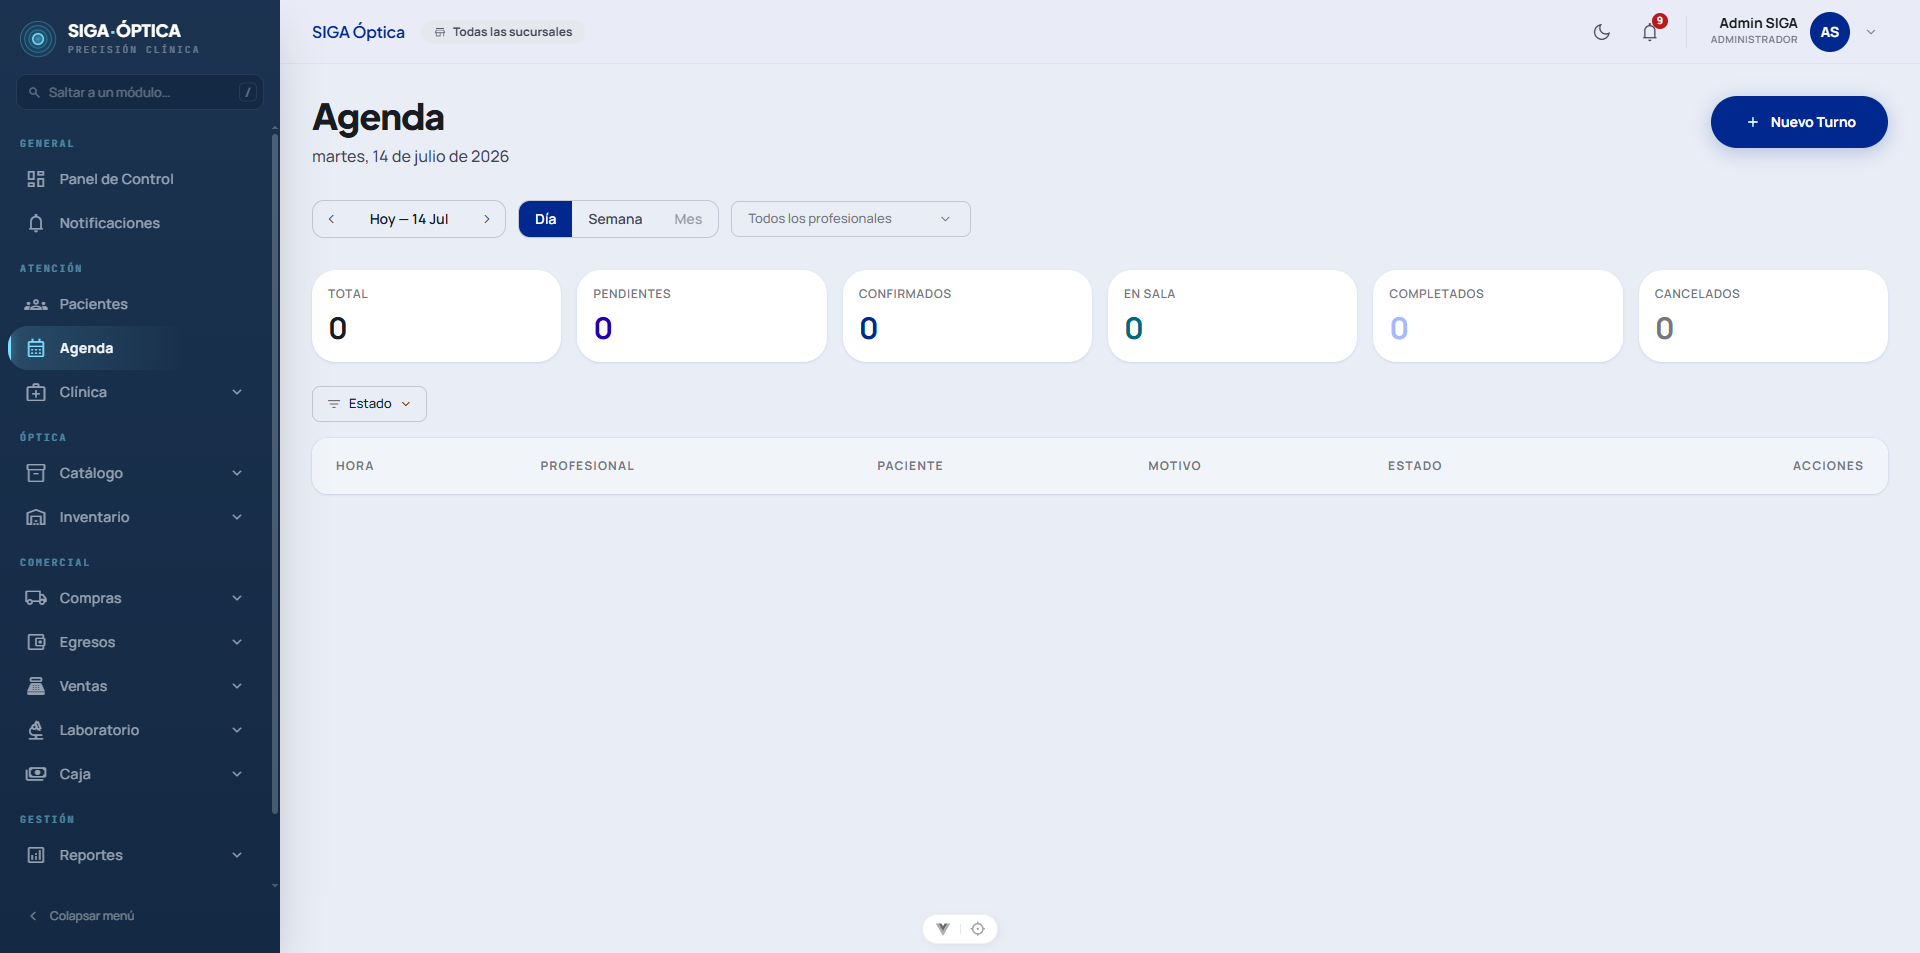
\includegraphics[width=0.95\textwidth]{../imagenes/mod04-agenda.png}
  \end{center}
\end{frame}

\begin{frame}{La aplicación --- historia clínica}
  \begin{center}
    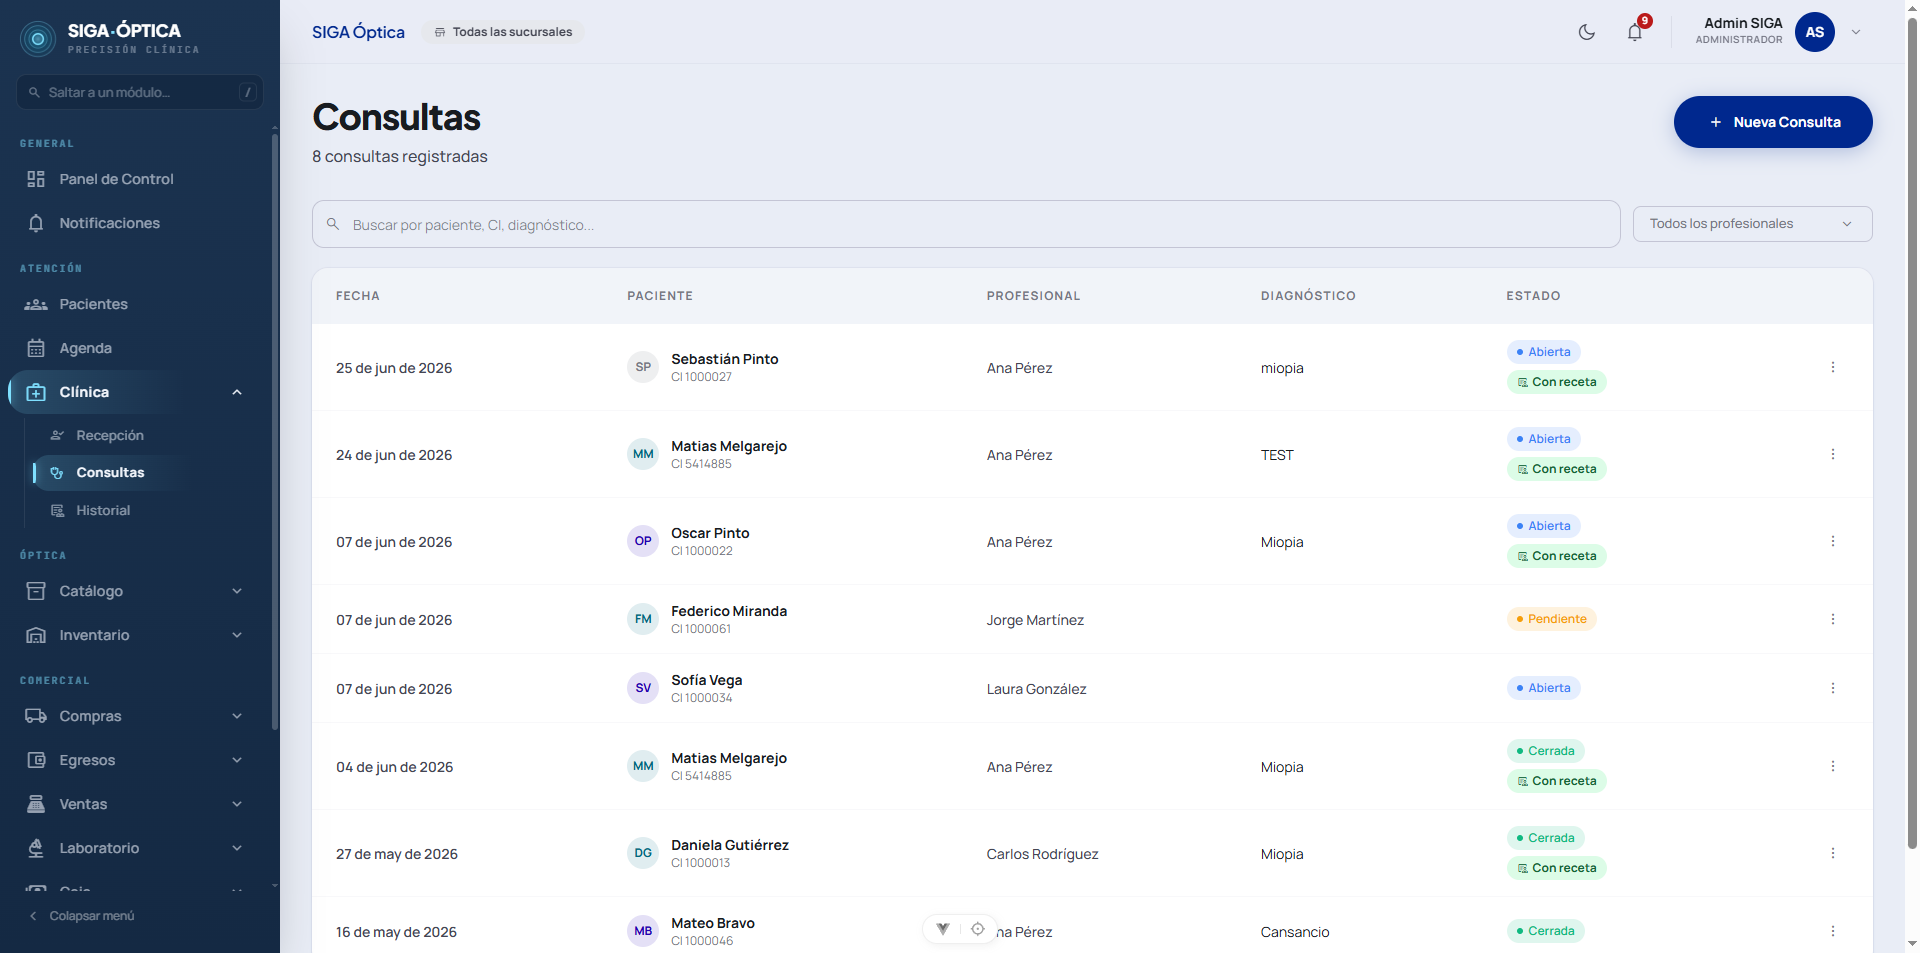
\includegraphics[width=0.95\textwidth]{../imagenes/mod05-clinica-consultas.png}
  \end{center}
\end{frame}

\begin{frame}{La aplicación --- ventas}
  \begin{center}
    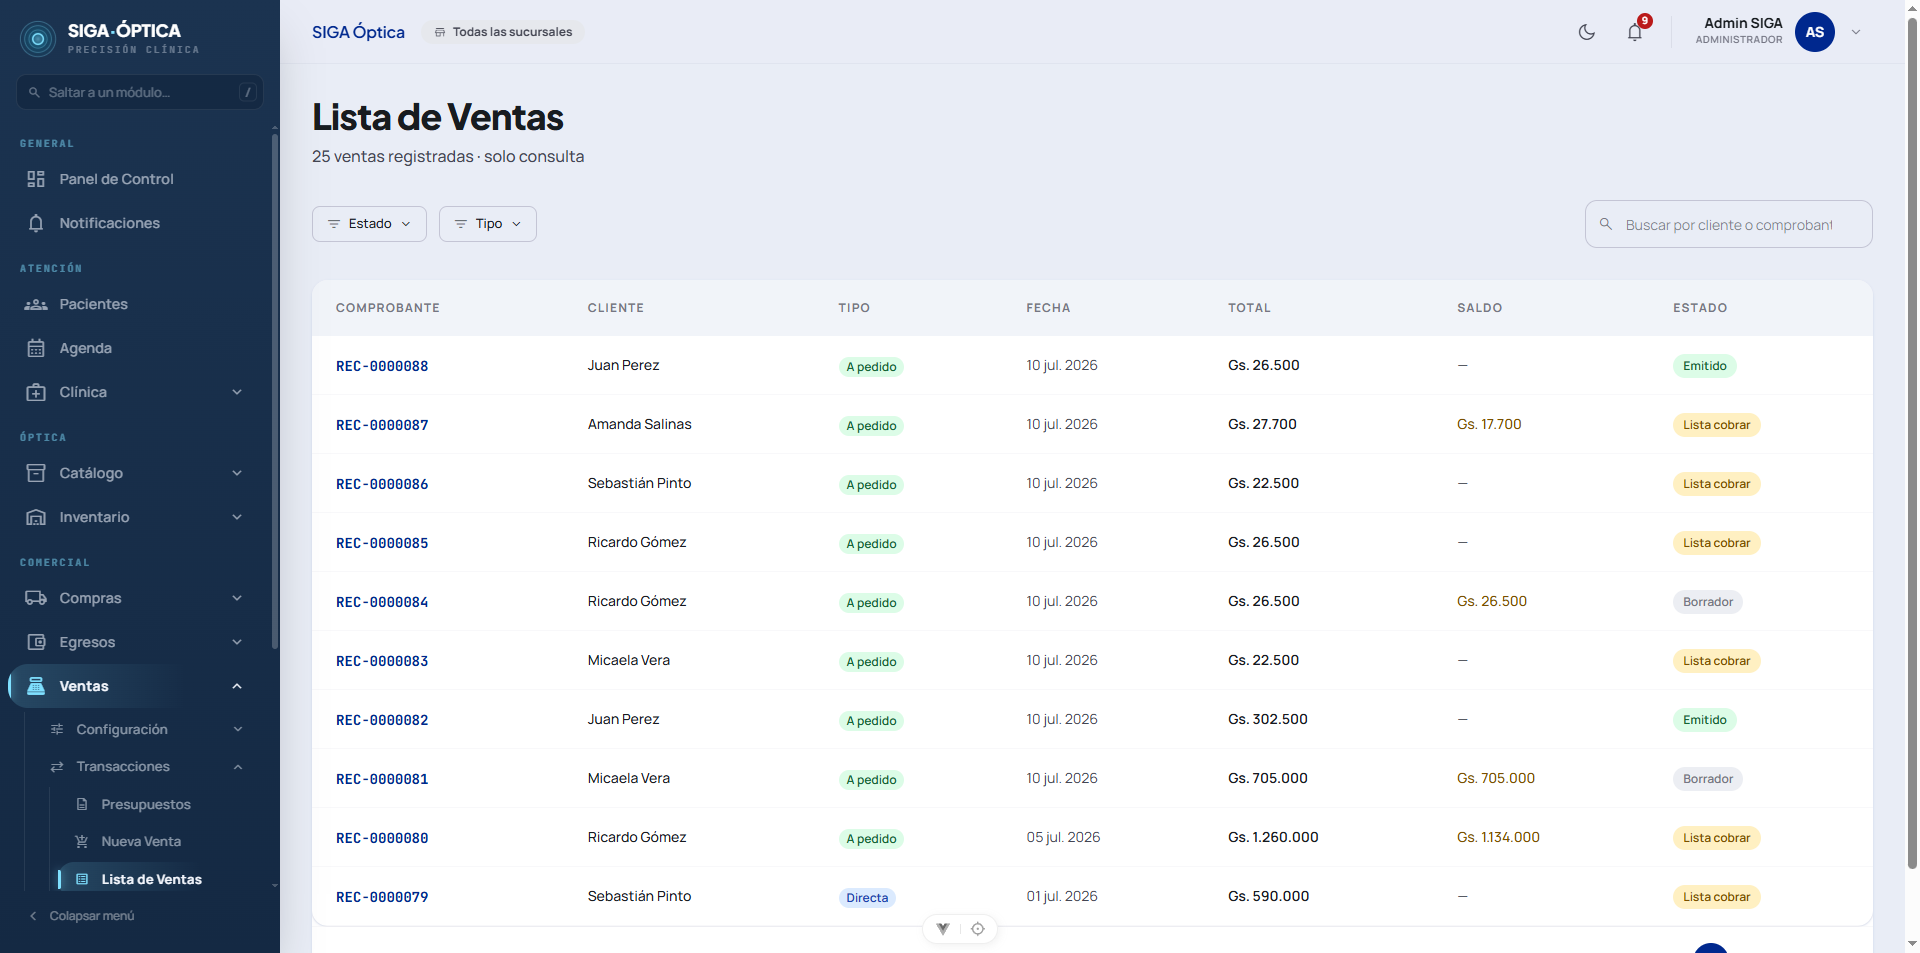
\includegraphics[width=0.95\textwidth]{../imagenes/mod08-ventas.png}
  \end{center}
\end{frame}

\begin{frame}{La aplicación --- reportes de gestión}
  \begin{center}
    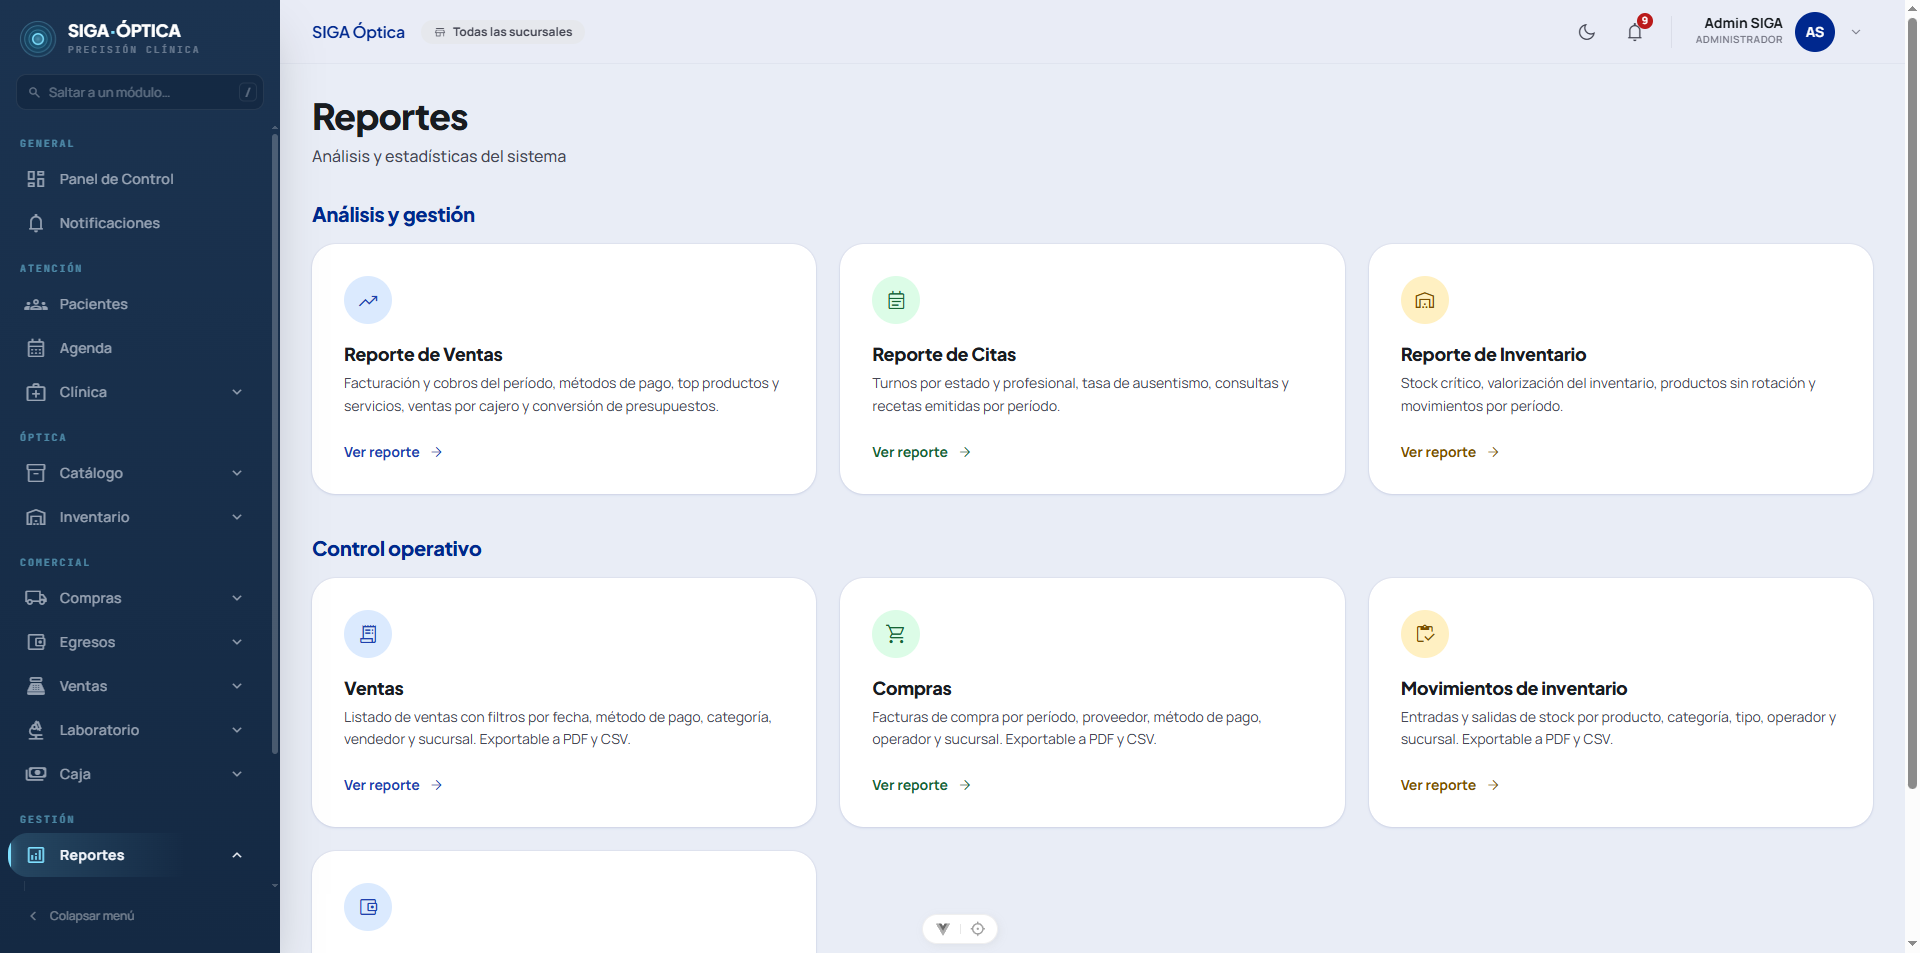
\includegraphics[width=0.95\textwidth]{../imagenes/mod14-reportes.png}
  \end{center}
\end{frame}

% ============================================================
\section{Cambios respecto al anteproyecto}

\begin{frame}{Cambios respecto al anteproyecto}
  \small
  \begin{tabular}{@{}p{4.2cm}p{9.4cm}@{}}
    \toprule
    \textbf{Planteado} & \textbf{Adoptado, y por qué} \\
    \midrule
    Sucursal como atributo del usuario
      & Sucursal como \textbf{entidad} con identidad propia: sin ella no hay stock ni caja por local. \\[3pt]
    Pedidos automáticos a proveedores
      & Reposición \textbf{asistida}: el sistema avisa el stock bajo y la persona decide. Comprometer dinero sin intervención humana no era aceptable para el negocio. \\[3pt]
    Cancelación autónoma del paciente
      & Cancelación en \textbf{dos pasos}: el paciente solicita, la óptica resuelve. Protege la agenda del profesional. \\[3pt]
    Vuetify como librería de componentes
      & \textbf{Sistema de diseño propio}: control total de la identidad visual y de la accesibilidad. \\[3pt]
    Notificación por correo, WhatsApp y SMS
      & \textbf{Centro de notificaciones interno + email}. WhatsApp y SMS exigen un proveedor contratado que la óptica no tiene. \\
    \bottomrule
  \end{tabular}
\end{frame}

% ============================================================
\section{Validación}

\begin{frame}{Cómo se validó el sistema}
  \begin{block}{Metodología}
    Validación \textbf{manual y end-to-end} contra la base de datos real, con el
    sistema corriendo: la API ejercitada con peticiones autenticadas con un token
    real, y el frontend conducido con \textbf{Playwright} sobre un navegador real.
  \end{block}

  \vspace{6pt}
  Cada módulo se validó con \alert{dos criterios simultáneos}:

  \vspace{4pt}
  \begin{enumerate}
    \item Que la operación produjera el \textbf{efecto esperado en la base de datos}
          --- no basta con una respuesta HTTP exitosa.
    \item Que ese efecto fuera \textbf{visible correctamente en la interfaz}.
  \end{enumerate}
\end{frame}

\begin{frame}{Resultados de la validación}
  \small
  \begin{tabular}{@{}p{5.0cm}p{8.6cm}@{}}
    \toprule
    \textbf{Qué se probó} & \textbf{Resultado} \\
    \midrule
    Aislamiento multi-sucursal
      & Un usuario no ve ni alcanza datos de otra sucursal; el administrador global sí. Sin regresión en los procesos de fondo. \\[3pt]
    Reglas de contraseña
      & Los cinco casos de la regla completa devolvieron lo esperado. \\[3pt]
    Migración de estados a enumerados
      & Mapeo verificado contra los datos reales antes de migrar; los flujos devolvieron idéntica respuesta después. \\[3pt]
    Unificación de escala monetaria
      & Confirmado que ningún registro perdía información con el cambio. \\[3pt]
    Reportes operativos
      & Las 8 combinaciones (4 reportes × PDF/CSV) generaron contenido real. \\
    \bottomrule
  \end{tabular}
\end{frame}

% ============================================================
\section{Conclusiones}

\begin{frame}{Objetivos alcanzados}
  \begin{itemize}
    \item[\textcolor{sigaVerde}{$\blacksquare$}] \textbf{Alcanzados.} Módulo de pacientes,
      módulo clínico digital y gestión de óptica con stock en tiempo real y registro
      de ventas.
    \item[\textcolor{sigaVerde}{$\blacksquare$}] \textbf{Alcanzado cualitativamente.}
      Interfaz consistente, responsive y accesible --- sin una medición formal de
      usabilidad que lo respalde con datos.
    \item[\textcolor{sigaAmbar}{$\blacksquare$}] \textbf{Parcial.} Agendamiento en línea:
      el paciente reserva y confirma de forma autónoma desde su navegador; no puede
      reprogramar, y la cancelación se resuelve en dos pasos.
    \item[\textcolor{sigaAmbar}{$\blacksquare$}] \textbf{No instrumentado.} La mejora
      del 20\% en eficiencia administrativa: el sistema no mide ese indicador, por lo
      que no puede darse por alcanzado ni por descartado.
  \end{itemize}
\end{frame}

\begin{frame}{Limitaciones conocidas}
  \begin{columns}[T,onlytextwidth]
    \begin{column}{0.49\textwidth}
      {\color{sigaAzul}\textbf{Alcance no implementado}}
      \begin{itemize}\small
        \item Reprogramación de citas.
        \item Adjuntar documentos y estudios a la consulta.
        \item Unificación de pacientes duplicados.
        \item Reporte comparativo de productividad entre profesionales.
        \item Segundo factor de autenticación.
      \end{itemize}
    \end{column}
    \begin{column}{0.49\textwidth}
      {\color{sigaAzul}\textbf{Del sistema construido}}
      \begin{itemize}\small
        \item Sin batería de pruebas automatizadas: la validación fue manual.
        \item Cambiar la contraseña no invalida las sesiones ya abiertas.
        \item Un solo canal externo de notificación (email).
        \item Stock mínimo y máximo global, no configurable por sucursal.
        \item Auditoría de cobertura curada: 15 acciones sensibles, no toda escritura.
      \end{itemize}
    \end{column}
  \end{columns}

  \vspace{6pt}
  {\small Se listan de forma explícita porque forman parte del alcance propuesto
  originalmente.}
\end{frame}

\begin{frame}{Trabajo futuro}
  \begin{itemize}
    \item \textbf{Pruebas automatizadas} sobre las reglas de negocio más sensibles:
      aislamiento por sucursal, cálculo de stock, reglas de cobro y facturación.
    \item \textbf{Canales de notificación adicionales} (WhatsApp, SMS), si la óptica
      contrata un proveedor.
    \item \textbf{Completar el módulo de notificaciones}: bitácora de envíos, aviso de
      retiro y plantillas administrables.
    \item \textbf{Refinar el soporte multi-sucursal}: stock mínimo/máximo por sucursal
      y selectores entre sucursales.
    \item \textbf{Instrumentar los indicadores de gestión} para medir con datos reales
      si el sistema mejora la eficiencia administrativa en la magnitud propuesta.
  \end{itemize}
\end{frame}

% ============================================================
{\setbeamertemplate{footline}{}
\begin{frame}[plain]
  \vfill
  \begin{center}
    {\LARGE\bfseries\color{sigaAzul}Gracias\par}
    \vspace{10pt}
    {\large ¿Preguntas?\par}
    \vspace{20pt}
    {\color{sigaAzul!30}\rule{0.35\textwidth}{0.8pt}}\\[12pt]
    {\small Matías Melgarejo \quad\textbullet\quad Matías Gaona\par}
    {\footnotesize\color{sigaGris}SIGA-Óptica --- Sistema Integral de Gestión y Agendamiento para Ópticas\par}
  \end{center}
  \vfill
\end{frame}}

\end{document}
